% -*- coding: utf-8 -*-

\subsection{tf.Variable}

\begin{frame}[fragile]
    \begin{tcblisting}{title=RefVariable的读写顺序问题}
        a = tf.Variable(1.0, use_resource=True)
        a.initializer.run()

        assign = a.assign(2.0)

        with tf.control_dependencies([assign]):
          b = a.read_value()

        with tf.control_dependencies([b]):
          other_assign = a.assign(3.0)

        with tf.control_dependencies([other_assign]):
          # Will print 2.0 because the value was read before other_assign ran. If
          # `a` was a tf.Variable instead, 2.0 or 3.0 could be printed.
          tf.Print(b, [b]).eval()
    \end{tcblisting}
\end{frame}

\begin{frame}{tf.Variable}
    The API for Variables will then change in the following ways for TF 2.0:\footnote{\href{https://github.com/tensorflow/community/pull/11}{RFC: Variables in TensorFlow 2.0}}

    \begin{itemize}
        \item RefVariable $\to$ ResourceVariable
        \item clean global scopes, and collections
            \begin{itemize}
                \item remove variable\_scope $\to$ name\_scope \\
                      graph.variable\_scope\_stack $\to$ module-global weak dict
            \end{itemize}
        \item tf.assign* will be removed
        \item get\_variable  $\to$ tf.Variable + scoped factory functions
    \end{itemize}
\end{frame}

\begin{frame}[fragile]
    \begin{tcblisting}{title=可能的常见用法}
        # 1. don't care
        a = tf.Variable(**kwargs)

        # 2.1 official subclass
        b_1 = ResourceVariable(**kwargs)

        def custom_creator(next_creator, **kwargs):
          return ResourceVariable(**kwargs)

        with tf.variable_creator_scope(custom_creator):
          b_2 = tf.Variable(**kwargs)
        assert b_1.eval() == b_2.eval()

        # 2.2 chain
        def custom_creator(next_creator, **kwargs):
          vars = [next_creator(**your_kwargs) for _ in range(3)]
          return PartitialedVariable(variable_list=vars, **kwargs)

        # 3. custom subclass
        class MyVariable(Variable):
          pass
    \end{tcblisting}
\end{frame}

\begin{frame}[fragile]
    \begin{tcblisting}{}
        def my_creator(next, **kwargs):
          return next(**kwargs)

        def other_creator(next, **kwargs):
          return next(**kwargs)

        def default_creator(next, **kwargs):
          if v1:
            return RefVariable(**kwargs)
          else:
            return ResourceVariable(**kwargs)

        creator_stack =[my_creator,
                        other_creator,
                        # ......
                        # ......
                        default_creator]

        # equal to
        def my_getter(**kwargs):
          return my_creator(
              other_creator(
                  default_creator(None, **kwargs),
                  **kwargs),
              **kwargs)

        my_variable = my_getter(**kwargs)
    \end{tcblisting}
\end{frame}

\begin{frame}[fragile]
    \begin{tcblisting}{title=tf.Variable and scoped factory function}
        class Graph(object):
          @tf_contextlib.contextmanager
          def _variable_creator_scope(self, creator):
            old = list(self._variable_creator_stack)
            self._thread_local._variable_creator_stack.append(creator)
            try:
              yield
            finally:
              self._thread_local._variable_creator_stack = old

        def _make_getter(captured_creator, previous_getter):
          return lambda **kwargs: captured_creator(previous_getter, **kwargs)

        # 封装到variable_scope.variable_creator_scope:
        with (ops.get_default_graph()
                 ._variable_creator_scope(custom_creator)):
          # 封装进tf.Variable:
          previous_getter = lambda **kwargs: default_variable_creator(None, **kwargs)
          for creator in ops.get_default_graph()._variable_creator_stack:
            previous_getter = _make_getter(creator, previous_getter),
          return previous_getter(**kwargs)

        # tf 2.0:
        with tf.variable_creator_scope(custom_creator):
          a = tf.Variable(**kwargs)
    \end{tcblisting}
\end{frame}

\begin{frame}[fragile]
    \begin{tcblisting}{}
        def creator_func(next_creator, **kwargs):
          pass

        def getter_func(**kwargs):
          pass

        my_getter = (
            lambda **k2:
                my_creator(
                    (lambda **k1:
                        other_creator(
                            (lambda **k0: default_creator(None, **k0)),
                    **k1)),
                **k2)),

        my_variable = my_getter(**kwargs)
    \end{tcblisting}

    \begin{align*}
        \operatorname{funcs} &= [f_0(g, x), f_1(g, x), \cdots, f_n(g, x)] \\
        g_0(x) &= f_0(\_, x)  \\
        g_n(x) &= f_n(g_{n-1}, x)  \quad \text{ For $n = 1, 2, \cdots, n$}
    \end{align*}
\end{frame}

\begin{frame}[fragile]
    \begin{columns}
        \begin{column}{.4\textwidth}
            \begin{figure}[!tb]
                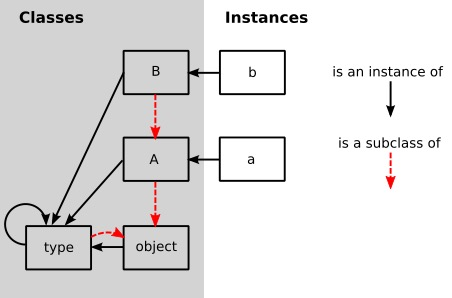
\includegraphics[width=\twopicwidth]{figure/var/metaclass}
                \caption{Python对象关系\footnotemark}
            \end{figure}
        \end{column}

        \begin{column}{.5\textwidth}
            \begin{tcblisting}{}
                class type(object):
                  def __call__(cls, *args, **kwargs):
                    obj = cls.__new__()
                    obj.__init__(*args, **kwargs)
                    return obj

                class A(object, metaclass=type):
                  pass

                A = type('A', (), {})

                class B(A):
                  pass

                B = type('B', (A,), {})

                a = A()
                a = super(A, cls).__call__()
            \end{tcblisting}
        \end{column}
    \end{columns}

    \footnotetext{\href{https://yq.aliyun.com/articles/226714}{用Python实现一个最简单的对象模型}}
\end{frame}

\begin{frame}
    \begin{figure}[!tb]
        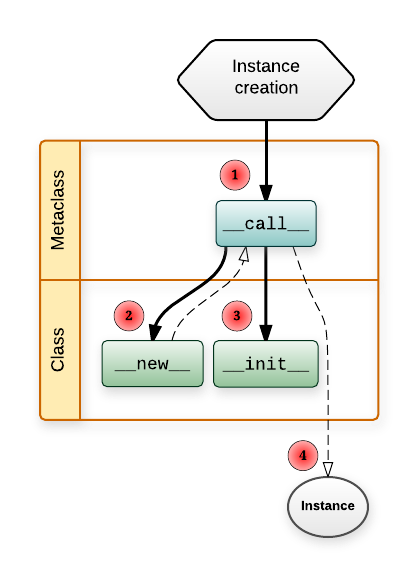
\includegraphics[width=0.7\onepicwidth]{figure/var/instance-creation}
        \caption{The diagram of how instances are constructed.\footnote{
                 \href{https://blog.ionelmc.ro/2015/02/09/understanding-python-metaclasses/}{Understanding Python metaclasses}}}
    \end{figure}
\end{frame}

\begin{frame}[fragile]
    \begin{tcblisting}{title=code snippet of tf 2.0 Variable}
            class VariableMetaclass(type):

              def _variable_v1_call(cls, **kwargs):
                pass

              def _variable_v2_call(cls, **kwargs):
                pass

              def __call__(cls, *args, **kwargs):
                if cls is VariableV1:
                  return cls._variable_v1_call(*args, **kwargs)
                elif cls is Variable:
                  return cls._variable_v2_call(*args, **kwargs)
                else:
                  return super(VariableMetaclass, cls).__call__(*args, **kwargs)

            @tf_export("Variable", v1=[])
            class Variable(six.with_metaclass(VariableMetaclass,
                                              checkpointable.CheckpointableBase)):
              def __init__(self, **kwargs):
                raise NotImplementedError
    \end{tcblisting}
    {\tiny \tt
    source: tensorflow/python/ops/variables.py \\[-2ex]
    commit: 4a5693e732b80a593bca7bf94ddd5df9e5d78cc0}
\end{frame}
